% =============================================================================
%  pic-tex/example-tikz/example-tikz.tex
%  FIGURE WRAPPER: includes the pre-compiled PDF (example-tikz-source.pdf)
%  produced from example-tikz-source.tex in the same folder. Input this file
%  from text/APPENDIX/figures.tex or any other place.
%  图片包装文件：插入同目录下由 example-tikz-source.tex 编译得到的 PDF。
% =============================================================================

\begin{figure}[htbp]
  \centering
  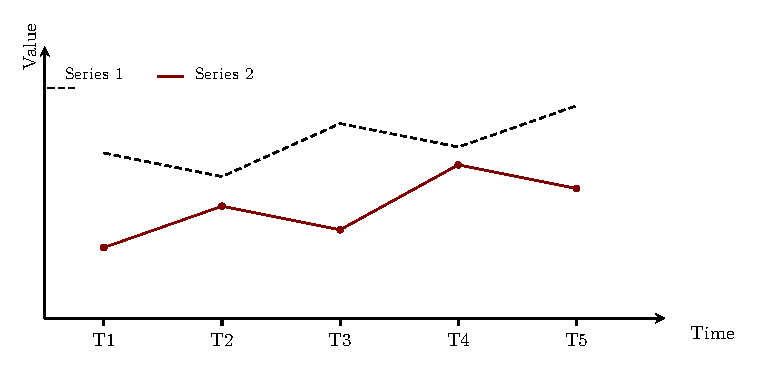
\includegraphics[width=0.8\textwidth]{pic-tex/example-tikz/example-tikz-source.pdf}
  \vspace{0.5em}
  \caption{A Generic Example Figure (Placeholder)}
  \label{fig:appendix-tikz}
  \vspace{0.5em}
  \caption*{\footnotesize \justifying \textit{Note:} This is a placeholder
  figure demonstrating the TikZ workflow. Compile
  \texttt{pic-tex/example-tikz/example-tikz-source.tex} to regenerate the
  PDF, then replace the drawing with your own content.}
\end{figure}
